HTBAC % by design 
allows to % represents 
encode binding free energy protocols, such as ESMACS and TIES, into ensemble
applications\@. We define a protocol as an ensemble of replicas where each
replica consists of an identical sequence of simulation stages.
\jhanote{I don't think this is a suitable description of how we model a
protocol: what is a simulation step? steps or stages?} \jdnote{@sj I
redefined simulation steps as simulation stages in the entire paper.}

We express the application logic of HTBAC using the user-facing API 
% components 
of EnTK (\S\ref{ssec:entk}). 
\jhanote{Why not use ensemble member as opposed to replica? ensemble --> the
collective; ensemble member --> a non-specific ensemble instance drawn from
the collective.} \jdnote{Earlier in methodology we refer to a replica as an
ensemble member.}
The EnTK % provides a common 
API and its programming model 
\jhanote{What programming model? EnTK's programming model?} \jdnote{changed
to the EnTK API and its programming model}
allow HTBAC to express the workflows associated with different protocols as
ensemble-based applications, % uniformly, and thus 
minimizing development effort and complexity.
% We describe these components for the ESMACS protocol\@. Typically, a
% protocol % typically corresponds to a single physical system.

The concept of % an 
ensemble of replicas in the ESMACS and TIES protocol directly maps to a set
of pipelines in EnTK, where each replica
\jhanote{replica of what?}\jdnote{I defined a replica earlier where each
replica consists of a sequence of simulations steps} maps to a single
pipeline consisting of a sequence of stages. Each stage consists of tasks
\mtnote{each stage has only one task as specified in the following paragraph}
that perform unique functions including preprocessing and molecular dynamics
simulations. \jhanote{Achtung: simulation steps will be confused with the
number of steps for an MD simulation} \jdnote{changed from sim step to sim
stage}

% directly to a set of pipelines in EnTK, where each pipeline contains
% functions that operate on a given replica. EnTK interprets these replicas
% as independent pipelines. Each pipeline consists of multiple stages
% representing a well-defined execution order; each stage can contain
% heterogeneous workloads. Although each stage of a pipeline depends on its
% predecessor, the pipelines execute independently of each other.
ESMACS and TIES protocols differ in the details of the pipelines, stages and
synchronization~\cite{Bhati2017}.
% The patterns
% \jhanote{what is a pattern within a pipeline? a pipeline is a pattern by
% some accounts?} within pipelines; however, are identical and describe an
% ensemble of replica simulations.
Fig~\ref{figure:HTBAC} % demonstrates 
shows how pipelines, stages and tasks are organized for the ESMACS
protocol.

% \mtnote{I am afraid we need to iterate the whole pragraph. We need to
% separate between the abstracitons used in the ESMACS protocol (replica,
% function, simulation) to those of EnTK (pipeline, stage and task). Once
% separated, we need to map the former into the latter.} \jdnote{better? also
% see caption of HTBAC figure}

\begin{figure}
\centering
  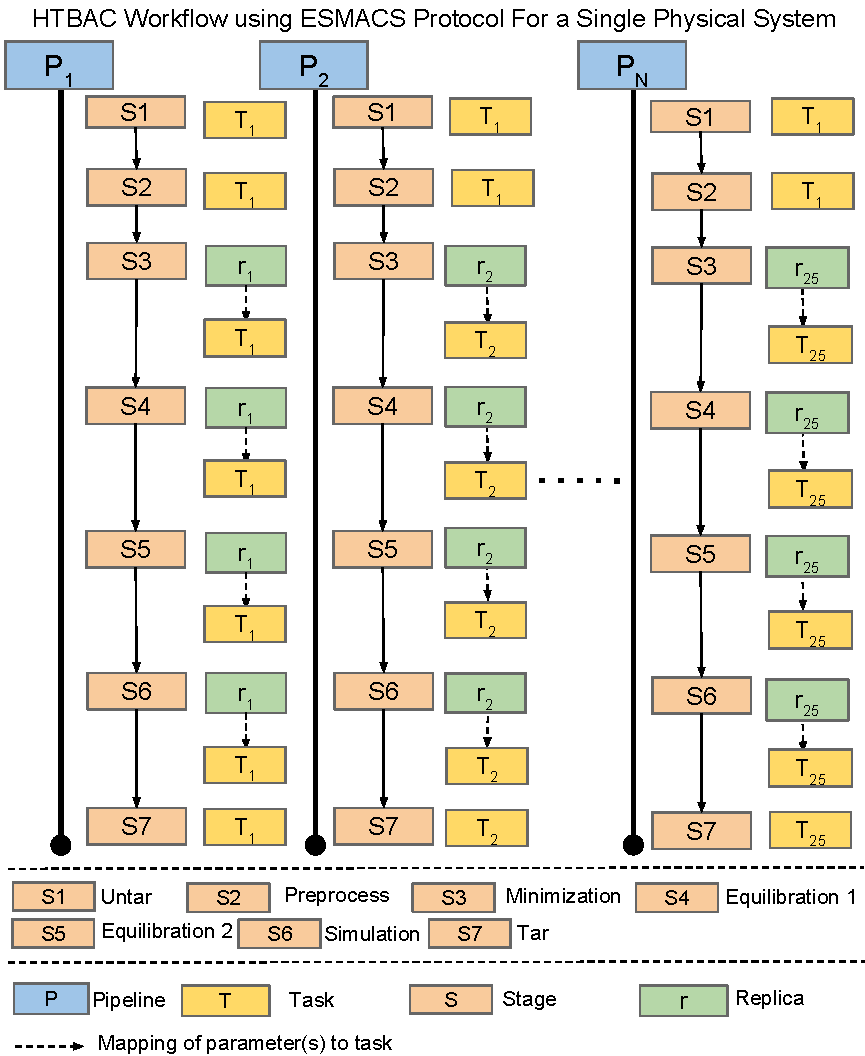
\includegraphics[width=0.5\textwidth]{FIGURES/HTBAC_Workflow_ESMACS.pdf}
  \caption{ESMACS protocol implemented as an HTBAC
  workflow\mtnote{application?}, encoded using the EnTK % PST model
  API\mtnote{PST model is not defined in this paper}. Each protocol
  represents a physical system and is % captured 
  encoded as a set of independent pipelines. Each pipeline maps to a single
  replica, where ESMACS consists of 25 replicas. Stages within a pipeline
  % maintain temporal ordering
  are executed sequentially. Each stage contains tasks \mtnote{each stage has
  only one task as specified in the following paragraph} performing unique
  functions, as required by the protocol. Stages S3--S6 contain molecular
  dynamics simulation tasks executed with NAMD\@.}\label{figure:HTBAC}
\end{figure}

% The ESMACS protocol consist of pipelines with stages comprised of
% heterogeneous tasks. For example, equilibration and production, followed by
% post processing steps. 

% \begin{figure}
% \centering
%   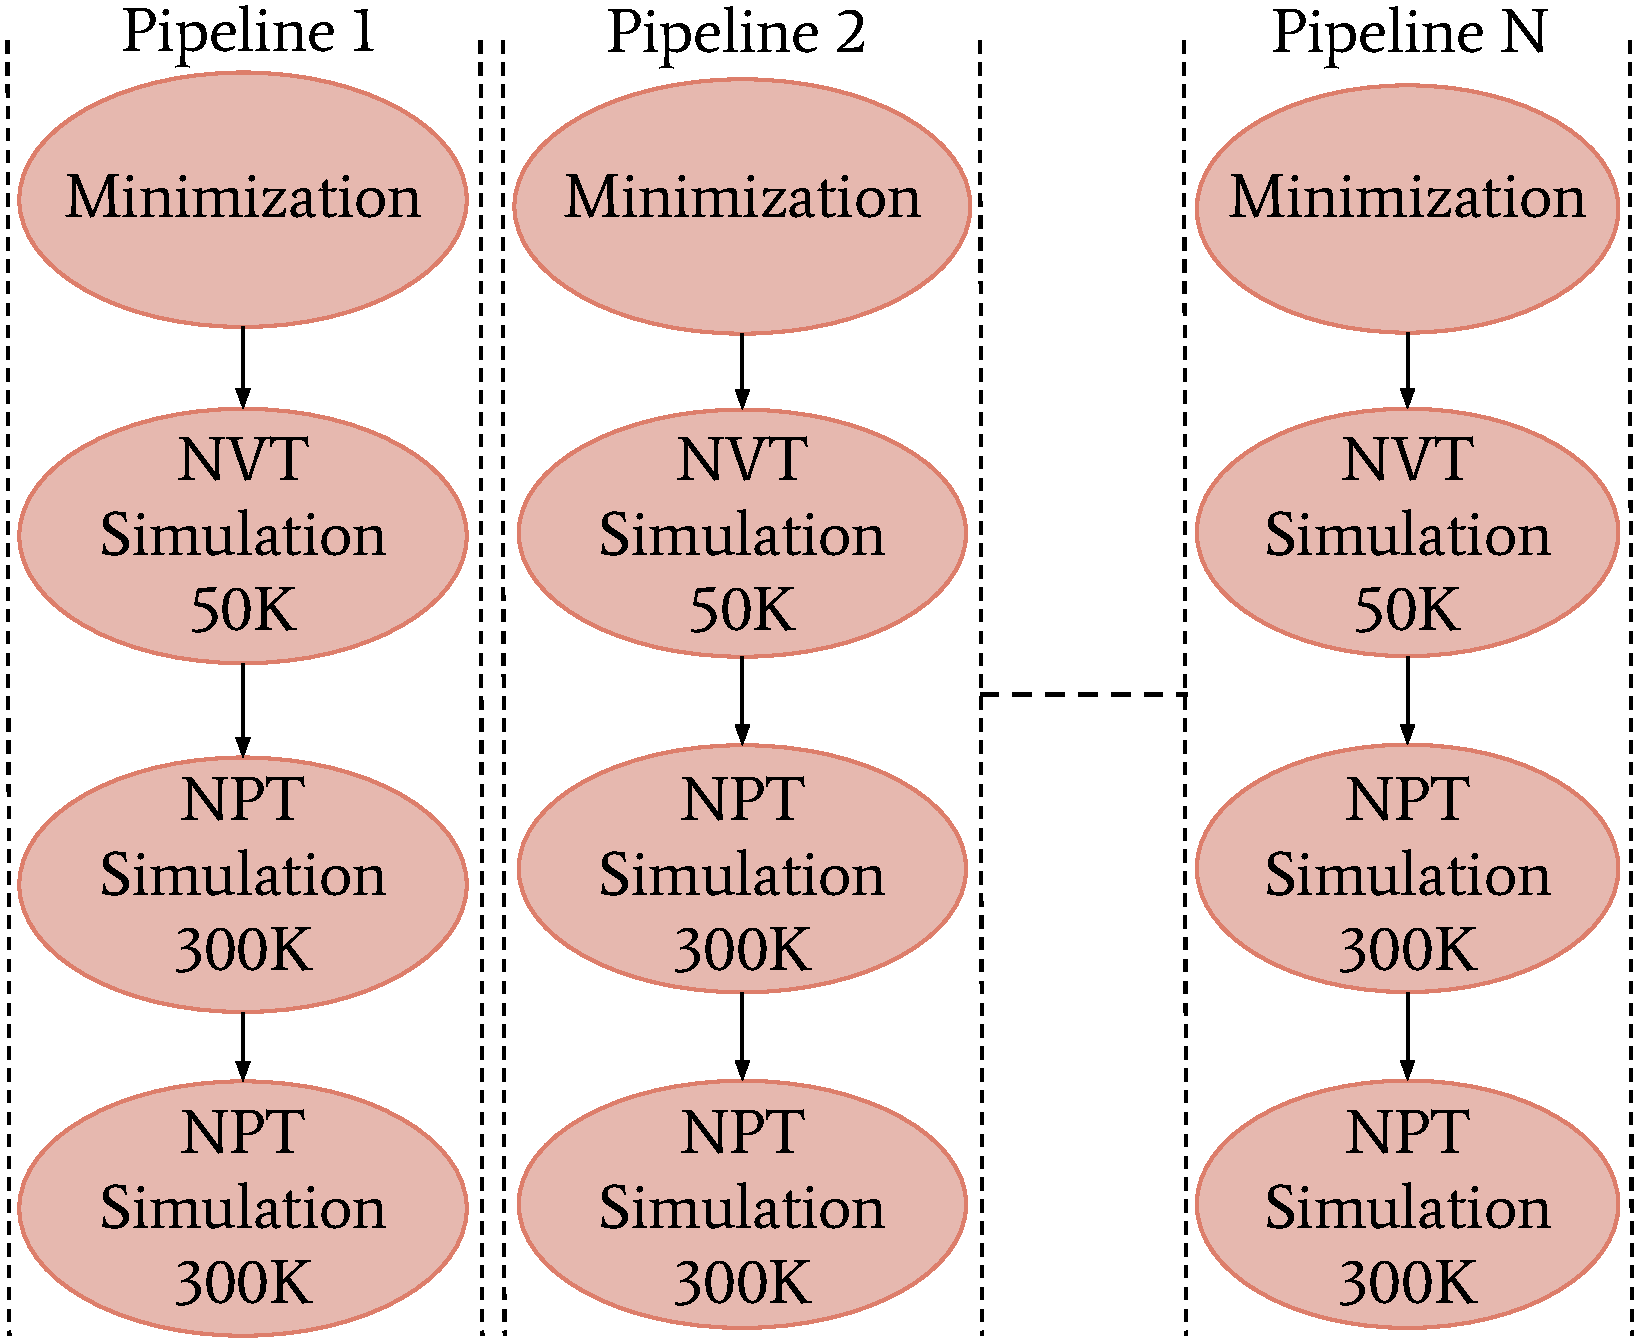
\includegraphics[width=0.5\textwidth]{FIGURES/HT-BAC_NAMD_pipelines_control_flow_only.pdf}
%   \caption{ESMACS protocol indicating how an N replica ensemble is implemented in HTBAC.
%   Each protocol instance is mapped to a single EnTK pipeline.
%   Each pipeline is equivalent and represents a set of simulations which are captured as stages by
%   EnTK.}\label{figure:ESMACS-pipelines}
% \end{figure}

%\begin{itemize}
%	\item 1) Untar configuration files
%	\item 2) Preprep
%	\item 3) Minimize with decreasing restraints
%	\item 4) Equilibration: NVT simulation at 50K, with restraints
%	\item 5) Equilibration: NPT simulation at 300K, with decreasing
%	restraints
%	\item 6) Equlibratin: NPT at 300k, no constraints
%	\item 7) Tarball output files
%\end{itemize}

Each stage is composed of a single % unique 
task with
% which is described by 
a set of attributes that define % the workload 
parameters % such as 
like the location of input files, the number of simulations and the MD
engine(s) used to launch those simulations. The ESMACS protocol % defines 
has 7 stages: %, in which 
the first and last stages perform staging of the input/output data, and the
middle stages indicate simulation tasks as shown in Fig~\ref{figure:HTBAC}.
The task is appended to a stage and stages are appended to a pipeline to
maintain temporal order. The workflow relies on a resource configuration
which consists of the details required to use a resource where the
application will be executed including runtime, queue, and account details.
We capture the integration of the application (ESMACS protocol) and how it
interfaces with EnTK in Fig~\ref{figure:ht-bac_rp}.

% \begin{figure}
% \centering
%   \includegraphics[width=0.5\textwidth]{FIGURES/HT-BAC_NAMD_pipelines_contr
%   ol_flow_only.pdf}
%   \caption{\bf NAMD Stages of HTBAC ESMACS protocol.}
%   \label{figure:ESMACS-pipelines}
% \end{figure}

We define the client resource in Fig~\ref{figure:ht-bac_rp} as the workload
system---HTBAC which describes a set of replicas with ordered functions as a
pipelines with stages and tasks. EnTK interprets these pipelines as a
functional set of tasks and generates the pilot description that contains the
resource configuration of how to run the HTBAC workload. For the ESMACS
protocol running on Blue Waters we define the runtime system, queue, and the
pilot size. Once RADICAL-Pilot receives this new workload it generates a
pilot that submits placeholders to the queue. Once the pilot is activated,
the RP-Agent submits the tasks in the form of compute units to the
placeholders to begin execution.

\begin{figure}
\centering
  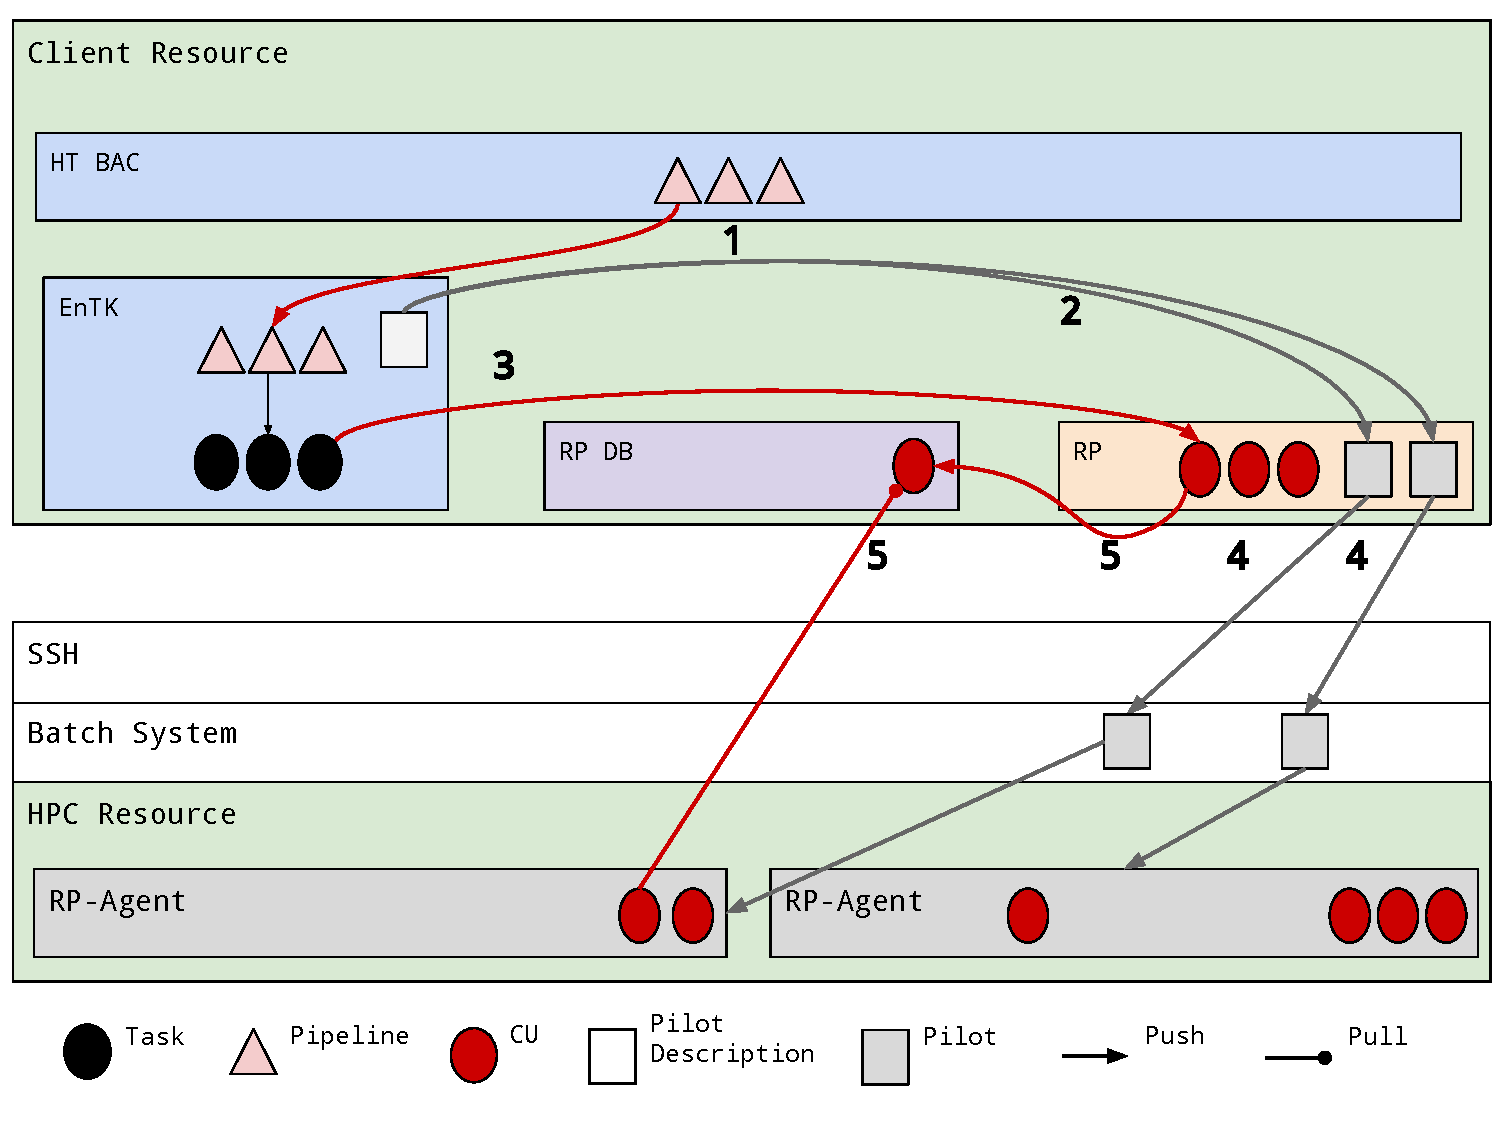
\includegraphics[width=0.5\textwidth]{FIGURES/ht-bac-rp_integration.pdf}
  \caption{Integration between HTBAC workflow and EnTK\@. Numbers indicate
  the temporal sequence of execution. The database (DB) of RADICAL-Pilot (RP)
  can be deployed on any host reachable from the resources. RP pushes compute
  units (CU) to DB and RP-Agent pulls them for execution. \dwwnote{I think CU
  needs to be defined here}\mtnote{Better?}}\label{figure:ht-bac_rp}
\end{figure}

RADICAL-Cybertools provides advanced resource management capabilities and,
thereby delivers the necessary high-throughput capabilities required. HTBAC
is integrated with the EnTK component of RCT.


% \begin{figure}[ht]
% \centering
%  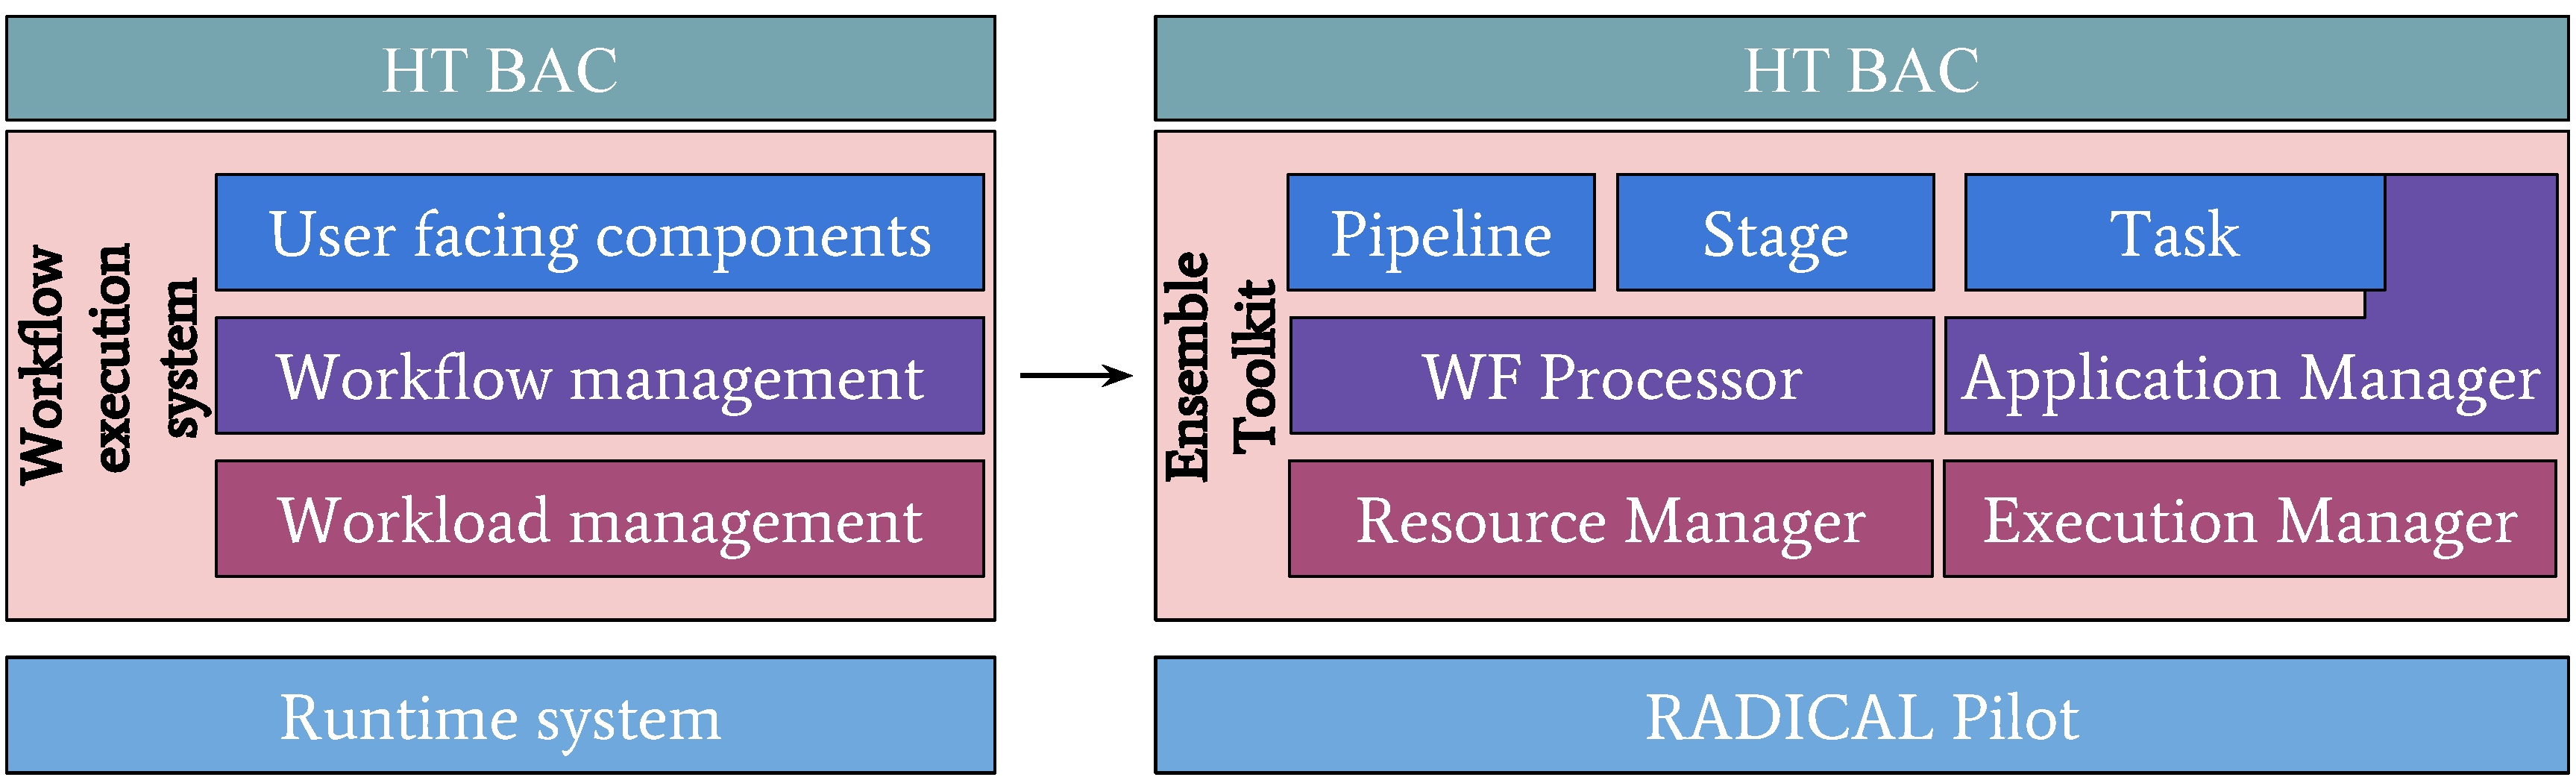
\includegraphics[width=0.5\textwidth]{FIGURES/entk_htbac_integration.pdf}
%   \caption{\bf Integration between HT-BAC workflow system and EnTK that
%   shows resource/application managers.}
%   \label{figure:ht-bac_entk}
% \end{figure}
